% TODO: Cleanup scalebox.
\documentclass[tikz]{standalone}
\usepackage{pgfplots}
\pgfplotsset{compat=1.15}
\usepackage{mathrsfs}
\usetikzlibrary{arrows,calc}
\usepackage{tkz-euclide}

\pagestyle{empty}

\definecolor{AngleClr}{rgb}{0,0.39215686274509803,0}
\definecolor{ShapeClr}{rgb}{0.6,0.2,0}

\begin{document}

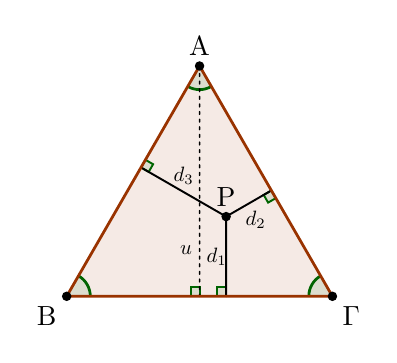
\begin{tikzpicture}[scale=.75]
\tkzSetUpLine[line width=1pt,color=black]
\tkzSetUpPoint[fill=black]

\tkzDefPoints{0/0/B,2.25/3.9/A,4.5/0/C,2.7/1.35/P}

\tkzDefPointBy[projection = onto A--B](P) \tkzGetPoint{PC}
\tkzDefPointBy[projection = onto A--C](P) \tkzGetPoint{PB}
\tkzDefPointBy[projection = onto B--C](P) \tkzGetPoint{PA}
\tkzDefPointBy[projection = onto B--C](A) \tkzGetPoint{HA}

\tkzFillPolygon[fill=ShapeClr,fill opacity=0.1](A,B,C)
\tkzFillAngles[fill=AngleClr,size=.4,fill opacity=0.1](C,B,A A,C,B B,A,C)
\tkzMarkAngles[line width=1pt,size=.4,color=AngleClr](C,B,A A,C,B B,A,C)

\tkzMarkRightAngles[line width=0.7pt, size=.15,color=AngleClr,fill=AngleClr,fill opacity=0.1](P,PA,B P,PB,C P,PC,A A,HA,B)


\tkzDrawSegment[line width=0.55pt,color=black,dashed,dash pattern=on 1pt off 1.75pt](A,HA)
\tkzDrawSegments[line width=0.7pt,color=black](P,PA P,PB P,PC)

\tkzDrawPolygon[color=ShapeClr](A,B,C)
\tkzDrawPoints[size=3](A,B,C,P)
\tkzLabelPoint[above](A){$\rm A$}
\tkzLabelPoint[below left](B){$\rm B$}
\tkzLabelPoint[below right](C){$\rm \Gamma$}
\tkzLabelPoint[above](P){$\rm P$}


\tkzLabelSegment[scale=0.75,left=-3pt](P,PA){$d_1$}
\tkzLabelSegment[scale=0.75,below](P,PB){$~~d_2$}
\tkzLabelSegment[scale=0.75,above](P,PC){$d_3$}

\tkzLabelSegment[scale=0.75,left, pos=0.8](A,HA){$~~~~u$}
\end{tikzpicture}

\end{document}
